\documentclass[12pt]{article}

\usepackage{CJK,graphicx}
\usepackage{fullpage}
\usepackage{epsfig}
\usepackage{amsfonts}
\usepackage{amssymb}
\usepackage{amstext}
\usepackage{amsmath}
\usepackage{xspace}
\usepackage{shadow,shadethm}
\usepackage{url}
%\usepackage[compact]{titlesec}
\usepackage{times}



\newcommand{\eqn}{\begin{eqnarray}}
\newcommand{\eqns}{\begin{eqnarray*}}
\newcommand{\uneq}{\end{eqnarray}}
\newcommand{\uneqs}{\end{eqnarray*}}

\newtheorem{theorem}{Theorem}
\newtheorem{lemma}{Lemma}
\newtheorem{claim}{Claim}
%\newtheorem{defn}[thm]{Definition}
\newtheorem{prop}[theorem]{Proposition}
\newcommand\ignore[1]{}
\def\tab{\hspace{5mm}}

\newenvironment{proof}
{\noindent{\bf Proof:}}
{\hfill\rule{2mm}{2mm}\medskip}

\newenvironment{proofof}[1]
{\noindent{\bf Proof of {#1}:}}
{\hfill\rule{2mm}{2mm}\medskip}

\newcommand{\problem}[1]{\vspace{0.4cm}\noindent{\bf Problem #1:}}
\newcommand{\Answer}{\vspace{0.4cm}\noindent{\bf Answer: }}

%-----document begins here-----

\title{Disease-target association prediction \\
}

%\author{Institute for Interdisciplinary Information Sciences, Tsinghua University}

\begin{document}
\date{}

\maketitle \vspace{-1cm}

%\setlength{\baselineskip}{18pt plus 1pt minus 1pt}

\setlength{\baselineskip}{18pt plus 1pt minus 1pt}




\section{Problem Description}

In this problem, your goal is to develop an algorithm to predict
disease-target associations based on the following two types of data:

\begin{enumerate}
\item[(1)] The interactions or associations between nodes in a
heterogeneous network depicting the relationships among drugs,
targets, diseases and drug side-effects. In particular, we have
linkages between drugs, proteins, diseases and side effects. The
specific graph depicting the relationship is shown in
Fig.~\ref{fig:network}.

\item[(1)]  The similarity scores between drugs or targets.
 Specifically, for chemicals (drugs), the scores are calculated
through Tanimoto coefficient using the product-graph of these two
structures~\cite{hattori2003development}. For targets, the scores
are computed using the simple Smith-Waterman
scores~\cite{smith1981identification} on genome sequences.
\end{enumerate}


\begin{figure}[h]
\centering
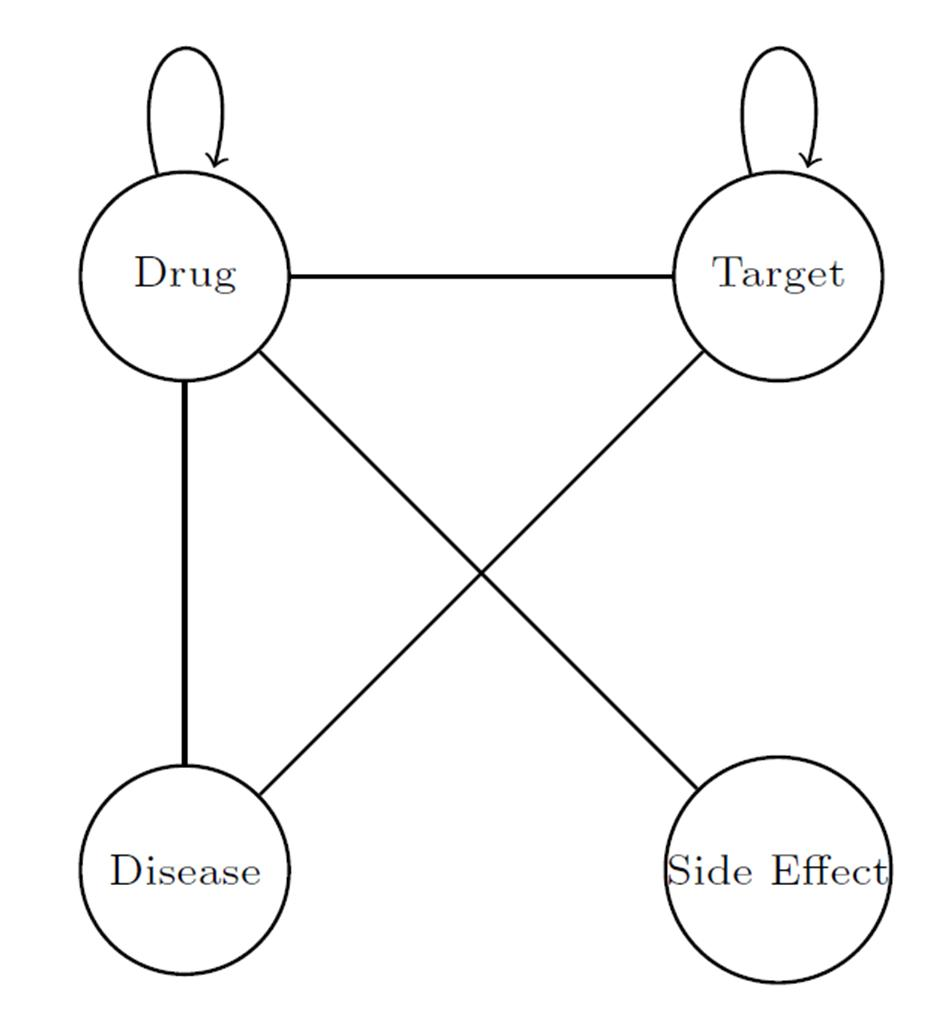
\includegraphics[width=90mm]{network.eps}
\caption{The schema of the heterogeneous
network.}\label{fig:network}
\end{figure}



There is one thing that needs to be specified  about the
interaction network data: the all-zero lines are very common in
the drug-target interaction matrix, that is, one drug (target) may
have no interaction with any one of the existed targets (drugs).

%The total statistics can be displayed as following:

%\begin{table}[H]
%\centering
%\begin{tabular}{cc}
%\toprule[1.5pt]
%\textbf{Data Type} &\textbf{Number of instances}\\
%\midrule
%  Drug &708\\
%  Protein &1512\\
%  Disease &5603\\
%  Side Effect &4192\\
%\bottomrule[1.5pt]
%\end{tabular}
%\caption{Number of elements for each data type}
%\end{table}

%\begin{table}[h]\footnotesize
%\centering
%\begin{tabular}{ccc}
%  \toprule[1.5pt]
%  \textbf{Interaction Type (Row-Column)} &\textbf{\# Zero rows/\# Total rows} &\textbf{\# Zero columns/\# Total columns}\\
%  \midrule
%  drug-disease  &0/708 &421/5603\\
%  drug-drug &136/708 &136/708\\
%  drug-se &0/708 &364/4192\\
%  protein-disease &0/1512 &1952/5603\\
%  protein-drug &1088/1512 &159/708\\
%  protein-protein &251/1512 &251/1512\\
%\bottomrule[1.5pt]
%\end{tabular}
%\caption{Interaction statistics}
%\end{table}



Implement your algorithm in any programming language that you are
familiar with, such as Java, C/C++, Matlab, etc., and then test
your algorithm on the given data. You are allowed to call any
other available public package in your program. If so, please
include the library in your final submission.


Use a cross-validation procedure to evaluate performance of your
algorithm. More details about cross-validation can be found in
wikipedia or other references. You can use the \emph{area under
receiver operating characteristic} (AUC) curve, the \emph{area
under the precision-recall} (AUPR) curve, or other measures to
assess the performance of your prediction method.

After running the cross-validation procedure, use the whole
dataset as training data to predict the new disease-target
associations. For each new association in your top prediction list
(e.g., top 10 predictions), use ``google" or ``google scholar" to
search the literature and check whether there exists any evidence
to support your prediction. If so, describe them in your report.


\section{Data}
In the the root folder,  \verb+drug_dict_map+ and
\verb+protein_dict_map+ suggest the (complete) real drug and
protein names corresponding to each name label used in subfolder
\verb+./InteractionData+'s specification files.

All the interaction and similarity data are organized in a normal
matrix-like format. And the specification data are just names
separated by carriage return \verb/\n/.

In the folder \verb+./InteractionData+, there are in total 6 kinds
of interactions between different entities, which are listed as
follows:

\begin{table}[htpb]
  \centering
  \begin{tabular}{lll}
    \verb/mat_drug_se.txt/ &:&Drug-SideEffect interaction matrix\\
    \verb/mat_protein_protein.txt/ &: &Protein-Protein interaction matrix\\
    \verb/mat_protein_drug.txt/ &: &Protein-Drug interaction matrix\\
    \verb/mat_drug_drug.txt/ &: &Drug-Drug interaction matrix\\
    \verb/mat_protein_disease.txt/ &:       &Protein-Disease interaction matrix\\
    \verb/mat_drug_disease.txt/ &:      &Drug-Disease interaction matrix
  \end{tabular}
\end{table}

Note that these matrices have been already preprocessed to be
perfectly matched to each other (e.g., the rows of drug-disease
interaction matrix, which are drugs, corresponds to exactly the
same drugs listed in the rows of protein-drug interaction matrix).
The corresponding list of the entities, i.e., the list of
diseases, drugs, proteins and side-effects are listed in the
following files:

\begin{table}[htpb]
  \centering
  \begin{tabular}{lll}
    \verb/disease.txt/ &: &Disease names\\
    \verb/drug.txt/ &: &Drug names\\
    \verb/protein.txt/ &: &Protein names\\
    \verb/se.txt/ &: &Side Effects
\end{tabular}
\end{table}

In the folder \verb+./SimilarityData+, the two matrices denote the
similarity scores within drugs and targets (proteins):

\begin{table}[htpb]
  \centering
  \begin{tabular}{lll}
    \verb/Similarity_Matrix_Drugs.txt/ &: &Drug similarity scores\\
    \verb/Similarity_Matrix_Proteins.txt/ &: &Protein similarity scores
  \end{tabular}
\end{table}

\textbf{Note:} (1) As these data are unpublished, please DO NOT
distribute these data outside this course. (2) These data are very
raw data, you can preprocess the data according to some
principles. If so, please describe the principles that you use.

\section{Requirement of Report}
In your final report, you should address the following points:

(1) Details of your algorithm, such as overview, pseudo-code (or
flow chart), etc.

(2) Performance evaluation of your algorithm.

(3) Discussion about strength and limitation of your algorithm.

(4) Description of your top prediction results using the whole
dataset as training data, and validation results from the
literature.

\section{Final Submission}
For final submission, you need to provide: (1) report; (2) source
code and binary executable file of your program, and a short
readme file that describes how to compile and run your program.

% \begin{thebibliography}{}
%{\footnotesize
%
%%%%
%
%
%%%%
%\bibitem[Bleakley and Yamanishi, 2009]{Bleakley2009}
%Bleakley, K. and Yamanishi, Y. (2009).
%\newblock Supervised prediction of drug-target interactions using bipartite local models.
%\newblock {\em Bioinformatics}, 25(18), 2397-2403.
%
%
%\bibitem[Chen \textit{et al.}, 2012]{Chen2012}
%Chen, X. {\em et al.} (2012).
%\newblock Drug-target interaction prediction by random walk on the heterogeneous network.
%\newblock {\em Molecular BioSystems}, 8(7), 1970-1978.
%
%
%
%%%%
%\bibitem[Cheng \textit{et al.}, 2012]{Cheng2012}
%Cheng, F.  {\em et al.} (2012).
%\newblock Prediction of drug-target interactions and drug repositioning via network-based inference.
%\newblock {\em PLoS computational biology}, 8(5), e1002503.
%
%%%%
%\bibitem[Ding \textit{et al.}, 2013]{Ding2013}
%Ding, H. {\em et al.} (2013).
%\newblock Similarity-based machine learning methods for predicting drug-target interactions: a brief review.
%\newblock {\em Briefings in bioinformatics}, bbt056.
%
%
%
%%%%
%\bibitem[Mei \textit{et al.}, 2013]{Mei2013}
%Mei, J. P. {\em et al.} (2013).
%\newblock Drug-target interaction prediction by learning from local information and neighbors.
%\newblock {\em Bioinformatics}, 29(2), 238-245.
%
%%
%
%
%
%
%
%%%%
%\bibitem[{van Laarhoven} \textit{et al.}, 2011]{vanLaarhoven2011}
%{van Laarhoven}, T. {\em et al.} (2011).
%\newblock Gaussian interaction profile kernels for predicting drug-target interaction.
%\newblock {\em Bioinformatics}, 27(21), 3036-3043.
%
%%%%
%
%%%%
%\bibitem[Xia \textit{et al.}, 2010]{Xia2010}
%Xia, Z. {\em et al.} (2010).
%\newblock Semi-supervised drug-protein interaction prediction from heterogeneous biological spaces.
%\newblock {\em BMC systems biology}, 4(Suppl 2), S6.
%
%
%
%%%%
%\bibitem[Yamanishi \textit{et al.}, 2008]{Yamanishi2008}
%Yamanishi, Y. {\em et al.} (2008).
%\newblock Prediction of drug-target interaction networks from the integration of chemical and genomic spaces.
%\newblock {\em Bioinformatics}, 24(13), i232-i240.
%
%
%
%
%}
%\end{thebibliography}

\bibliographystyle{plain}
\bibliography{bib}
\end{document}
